\documentclass[a4paper,10pt]{article}
\usepackage[T1]{fontenc}
\usepackage[utf8]{inputenc}
\usepackage[english]{babel}
\usepackage{lmodern}
\usepackage[top=1.6cm,bottom=1.8cm,left=1.9cm,right=1.9cm]{geometry}
\usepackage{titlesec,enumitem,xcolor,graphicx,lastpage,fancyhdr}
\usepackage{fontawesome5}
\usepackage[hidelinks]{hyperref}

\hypersetup{colorlinks=true,urlcolor=blue!70!black,linkcolor=blue!70!black}
\pagestyle{fancy}\fancyhf{}\renewcommand{\headrulewidth}{0pt}
\fancyfoot[C]{\small\color{gray}Page \thepage\ of \pageref{LastPage}}
\setlength{\parindent}{0pt}

\titleformat{\section}{\large\bfseries\color{blue!70!black}}{}{0em}{}[\vspace{-0.7em}\rule{\textwidth}{0.5pt}]
\titlespacing{\section}{0pt}{9pt}{5pt}
\setlist[itemize]{leftmargin=1.1em,itemsep=2pt,topsep=2pt,parsep=0pt}
\newcommand{\role}[4]{\vspace{3pt}\noindent\hspace{0.6em}\parbox[t]{0.38\textwidth}{\raggedright\textbf{#1}}\hfill\parbox[t]{0.58\textwidth}{\raggedleft\textit{#2}}\\{\textit{#3}\hfill\textit{#4}}\vspace{1pt}}

\begin{document}
\noindent
\begin{minipage}[t]{0.78\textwidth}
\vspace{0pt}
{\huge\bfseries Prabhavit Gupta}\\[8pt]
{\small \faPhone\ +39-351-610-7807 \quad \faEnvelope\ \href{mailto:prabhavitg@gmail.com}{prabhavitg@gmail.com} \quad \faLinkedin\ \href{https://www.linkedin.com/in/prabhavit/}{Linkedin} \quad \faMapMarker*\ Venice, Italy}
\end{minipage}\hfill
\begin{minipage}[t]{0.18\textwidth}
\vspace{0pt}\raggedleft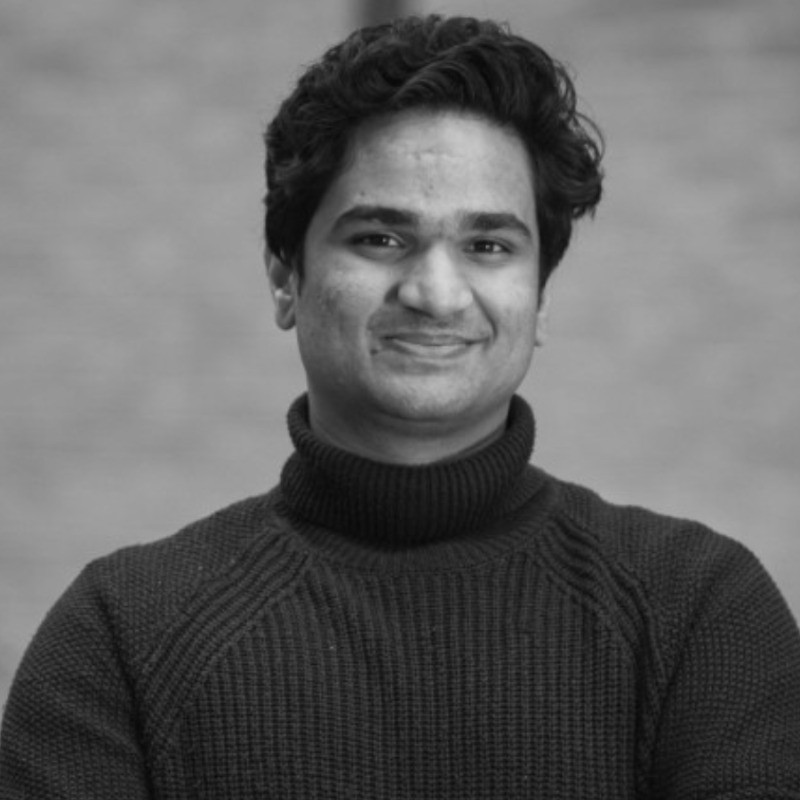
\includegraphics[width=2.3cm,height=2.3cm,keepaspectratio]{photo.jpg}
\end{minipage}

\section{Career Summary}
\begin{itemize}
\item Process Automation \& AI Specialist with hands-on experience architecting end-to-end intelligent automations combining RPA (UiPath), autonomous AI agents (Claude, LangChain), and API pipelines.
\item Proficient in evaluating operational workflows to engineer hybrid solutions---integrating deterministic RPA with generative AI, document understanding, and custom Python integration scripts.
\item Proven track record in full lifecycle deployment: technical scoping with cross-functional stakeholders, solution architecture, testing, exception handling, and ongoing performance tuning.
\end{itemize}

\section{Technical Skills}
\begin{itemize}
\item \textbf{Automation \& RPA} -- UiPath, Process Automation, n8n, Playwright, Exception Handling, Queue Management
\item \textbf{AI/ML \& Agents} -- AI Agents (Claude, LangChain), Document Understanding, NLP, RAG, OpenAI/Claude APIs, Eden AI
\item \textbf{Development} -- Python (custom integrations, scripting), TypeScript, REST/SOAP APIs, Laravel, SQL, Postman
\item \textbf{Architecture/DevOps} -- Solution Architecture, Version Control (GitHub), Jira, CI/CD, Figma
\end{itemize}

\section{Visa \& Language}
\begin{itemize}
\item \textbf{Language} -- English (Professional), Italian (Conversational), Hindi (Native)
\item \textbf{Work Authorization} -- European Long Term Residence Permit - No Sponsorship required. Open to hybrid work in Malta.
\end{itemize}

\section{Professional Experience}
\role{\href{https://flowspace.co}{FlowSpace.co}}{Lead Developer (Full time, Freelance)}{London, UK}{Mar 2024 -- Ongoing}
\begin{itemize}
\item \textbf{Product Responsibilities:}
\begin{itemize}[label=--]
\item Scaled platform from 2000 to 4500+ users through iterative product development
\item Overseeing the migration of app from Bubble.io to Next.JS and Laravel
\item Collaborated with team of developers for product logic and business logic documentation
\item Facilitated communication between internal team and Agency
\item Streamlined customer support with AI agents
\end{itemize}
\item \textit{Tools: Playwright, Jira, GoogleSheet, Clickup, Miro, Google Analytics, Microsoft Clarity}
\item \textbf{Technical Responsibilities:}
\begin{itemize}[label=--]
\item AI tool for processing and scraping of data and increasing listings on platform
\item Integration of external APIs (Office Rnd and Nexudus) for automated bookings
\item Consolidated leads in CRM and automated lead capture by developing integration between CRM used by the organization
\item GTM automations for sales funnel, lead enrichment and outbound
\item AI tool for processing of data and increasing listings on platform
\item Overseeing the migration of app from Bubble.io to Next.JS and Laravel
\item Developed a tool for companies to calculate commute times
\item \textit{Tools: Claude Code, n8n, Bubble.io, Postman, Jira, Github, Laravel, Typescript}
\end{itemize}
\end{itemize}

\role{Urlink}{Project Manager and AI Assisted Developer (Freelance)}{Barcelona, Spain}{April 2025 -- July 2025}
\begin{itemize}
\item Using AI for building the platform and logics
\item Implementing UIs made with AI
\item Implementing automations in regards to client requirements
\item \textit{Tools: Github, Netlify, Supabase, bolt.new}
\end{itemize}

\role{UltraStrategy.com}{Automation Developer (Collaborator)}{France}{Dec 2024 -- May 2025}
\begin{itemize}
\item Made a CV parsing tool using n8n and Eden AI
\item Developed platform for different user profiles
\item \textit{Tools: n8n, Eden AI, Bubble.io}
\end{itemize}

\role{Qomodo}{AI and Low-Code Developer (Collaborator)}{Milan, Italy}{2024 -- Jan 2025}
\begin{itemize}
\item Implementation of Figma designs
\item Made a dashboard to be used by the companies to manage their branches
\item \textit{Tools: Bubble}
\end{itemize}

\role{Get2Germany.com}{Lead Developer and Automation Specialist (Part time)}{Berlin, Germany}{Jan 2024 -- May 2024}
\begin{itemize}
\item Integration of Google APIs for effective tracking of the platform
\item UI/UX work, design from Figma to Bubble
\item Building the platform, database optimization
\item Developed AI based automation tools for finding courses, internships and jobs
\item \textit{Tools: Bubble.io, Figma, Trello, n8n}
\end{itemize}

\role{Clubee.com}{Low Code Developer and Quality Assurance (Full time, Freelance)}{Foetz, Luxembourg}{Sep 2023 -- Aug 2024}
\begin{itemize}
\item Integration of Clubee API for all of frontend
\item Unit testing and quality assurance of new features
\item Developed tools for: domain integration, shop, federation dashboard
\item \textit{Tools: Bubble.io, Figma, GitHub, Postman}
\end{itemize}

\role{Tractionboard.co}{Low-Code Developer (Internship)}{Utrecht, Netherlands}{Aug 2023 -- Oct 2023}
\begin{itemize}
\item ChatGPT/OpenAI integration
\item Implementation of designs from Figma to Bubble
\item Implementation of Sendgrid
\item Responsive designs, de-bugging
\item Google Ads 4 implementation
\item \textit{Tools: Bubble.io, Figma, Sendgrid, ChatGPT}
\end{itemize}

\section{Education}
\role{Ca' Foscari University of Venice}{Bachelor's in Philosophy, International Studies \& Economics with Minor in Entrepreneurship}{Venice, Italy}{Oct 2020 -- Jun 2024}

\section{Certifications}
\begin{itemize}
\item Microsoft Power Automate
\item Microsoft Copilot Studio Agent Academy
\item Microsoft - Introduction to building AI agents
\item Tray.AI Build Practitioner -- September 2024
\item Tray.AI Build Foundations
\end{itemize}

\end{document}
